
%(BEGIN_QUESTION)
% Copyright 2015, Tony R. Kuphaldt, released under the Creative Commons Attribution License (v 1.0)
% This means you may do almost anything with this work of mine, so long as you give me proper credit

This CEMS has a problem, and you are called to diagnose it.  The CO and NO$_{x}$ analyzers are reading too low, and the O$_{2}$ analyzer is registering too high (nearly 14\%, where its typical reading is 3\% or less):

$$\includegraphics[width=15.5cm]{i03729x01.eps}$$

The first thing you check are the rotameters.  The bypass flow registers a normal amount, while the span gas flow rate registers about half-scale.  You wait for 15 minutes to see if anything changes, but both rotameters keep reading the same steady flow rates.

Identify the likelihood of each specified fault for this sample system.  Consider each fault one at a time (i.e. no coincidental faults), determining whether or not each fault could independently account for {\it all} measurements and symptoms in this system.

% No blank lines allowed between lines of an \halign structure!
% I use comments (%) instead, so that TeX doesn't choke.

$$\vbox{\offinterlineskip
\halign{\strut
\vrule \quad\hfil # \ \hfil & 
\vrule \quad\hfil # \ \hfil & 
\vrule \quad\hfil # \ \hfil \vrule \cr
\noalign{\hrule}
%
% First row
{\bf Fault} & {\bf Possible} & {\bf Impossible} \cr
%
\noalign{\hrule}
%
% Another row
Valve $V_1$ shut &  &  \cr
%
\noalign{\hrule}
%
% Another row
Valve $V_7$ shut &  &  \cr
%
\noalign{\hrule}
%
% Another row
Valve $V_8$ shut &  &  \cr
%
\noalign{\hrule}
%
% Another row
Regulator $R_1$ failed high pressure &  &  \cr
%
\noalign{\hrule}
%
% Another row
Regulator $R_6$ failed low pressure &  &  \cr
%
\noalign{\hrule}
%
% Another row
Solenoid valve $S_4$ stuck open &  &  \cr
%
\noalign{\hrule}
%
% Another row
Solenoid valve $S_6$ stuck ``on'' &  &  \cr
%
\noalign{\hrule}
} % End of \halign 
}$$ % End of \vbox

Finally, identify the {\it next} diagnostic test or measurement you would make on this system.  Explain how the result(s) of this next test or measurement help further identify the location and/or nature of the fault.

\filbreak

\vskip 20pt \vbox{\hrule \hbox{\strut \vrule{} {\bf Suggestions for Socratic discussion} \vrule} \hrule}

\begin{itemize}
\item{} What significance is there in the fact that the bypass flow rate is normal?  In other words, what faults are ruled out by this fact, and what faults might still be possible in light of this fact?
\item{} Explain the purpose of the {\it chilled water bath} in this sample system.
\item{} Explain how this CEMS analyzer array is set up to be {\it self-calibrating}.
\item{} Can you identify any other possible faults not listed in the table which could account for all we're seeing?
\end{itemize}


\underbar{file i03729}
%(END_QUESTION)





%(BEGIN_ANSWER)


%(END_ANSWER)





%(BEGIN_NOTES)

% No blank lines allowed between lines of an \halign structure!
% I use comments (%) instead, so that TeX doesn't choke.

$$\vbox{\offinterlineskip
\halign{\strut
\vrule \quad\hfil # \ \hfil & 
\vrule \quad\hfil # \ \hfil & 
\vrule \quad\hfil # \ \hfil \vrule \cr
\noalign{\hrule}
%
% First row
{\bf Fault} & {\bf Possible} & {\bf Impossible} \cr
%
\noalign{\hrule}
%
% Another row
Valve $V_1$ shut &  & $\surd$ \cr
%
\noalign{\hrule}
%
% Another row
Valve $V_7$ shut &  & $\surd$ \cr
%
\noalign{\hrule}
%
% Another row
Valve $V_8$ shut &  & $\surd$ \cr
%
\noalign{\hrule}
%
% Another row
Regulator $R_1$ failed high pressure &  & $\surd$ \cr
%
\noalign{\hrule}
%
% Another row
Regulator $R_6$ failed low pressure &  & $\surd$ \cr
%
\noalign{\hrule}
%
% Another row
Solenoid valve $S_4$ stuck open & $\surd$ &  \cr
%
\noalign{\hrule}
%
% Another row
Solenoid valve $S_6$ stuck ``on'' &  & $\surd$ \cr
%
\noalign{\hrule}
} % End of \halign 
}$$ % End of \vbox

The most likely problem here is that ambient air is somehow entering the system and contaminating the process sample.  The fact we have flow through the span gas rotameter pretty much limits this air source to the span gas subsystem.  If it weren't for that rotameter indication, other sources wuch as tubing leaks anywhere upstream of the sample pump (where the partial vacuum would cause ambient air to enter the line through a leak) would be possible.



\vskip 20pt \vbox{\hrule \hbox{\strut \vrule{} {\bf Virtual Troubleshooting} \vrule} \hrule}

This question is a good candidate for a ``Virtual Troubleshooting'' exercise.  Presenting the diagram to students, you first imagine in your own mind a particular fault in the system.  Then, you present one or more symptoms of that fault (something noticeable by an operator or other user of the system).  Students then propose various diagnostic tests to perform on this system to identify the nature and location of the fault, as though they were technicians trying to troubleshoot the problem.  Your job is to tell them what the result(s) would be for each of the proposed diagnostic tests, documenting those results where all the students can see.

During and after the exercise, it is good to ask students follow-up questions such as:

\begin{itemize}
\item{} What does the result of the last diagnostic test tell you about the fault?
\item{} Suppose the results of the last diagnostic test were different.  What then would that result tell you about the fault?
\item{} Is the last diagnostic test the best one we could do?
\item{} What would be the ideal order of tests, to diagnose the problem in as few steps as possible?
\end{itemize}

%INDEX% Measurement, analytical: sample conditioning

%(END_NOTES)

